\documentclass[12pt,abstracton]{scrartcl}
%packages
\usepackage{bbm}
\usepackage{amssymb}
\usepackage{amsthm}
\usepackage{latexsym}
\usepackage{amsfonts}
\usepackage{amsmath}
\usepackage{texdraw}
\usepackage{euscript}
\usepackage{graphicx}
\usepackage{multirow}
\usepackage{mathrsfs}
\usepackage{textcomp}
\usepackage{color}
\usepackage{fancyvrb}
\usepackage{pstricks,pst-node,pst-tree}
\usepackage{subfig}
\usepackage{tikz}
\usepackage{url}
\usepackage{array}
%margins
\setlength{\textwidth}{6.5in}
\setlength{\evensidemargin}{0in}
\setlength{\oddsidemargin}{0in}
\setlength{\textheight}{9in}
\setlength{\topmargin}{-1in}
%section start markers
\newcommand{\lem}{\paragraph*{Lemma:}}
\newcommand{\cor}{\paragraph*{Corollary:}}
\newcommand{\prb}[1]{\section*{Problem {\text{#1}:}}}
\newcommand{\sprb}[1]{\subsection*{Item {\text{#1}:}}}
%abbreviations
\newcommand{\fa}{\forall}
\newcommand{\EE}{\exists}
\newcommand{\ee}{\epsilon}
\newcommand{\dd}{\delta}
\newcommand{\rr}{\mathbb{R}}
\newcommand{\rrx}{\rr^{\times}}
\newcommand{\qq}{\mathbb{Q}}
\newcommand{\nn}{\mathbb{N}}
\newcommand{\zz}{\mathbb{Z}}
\newcommand{\cc}{\mathbb{C}}
\newcommand{\ccx}{\cc^{\times}}
\newcommand{\oo}{\mathbb{O}}
\newcommand{\hh}{\mathbb{H}}
\newcommand{\pp}{\mathbb{P}}
\newcommand{\prm}[1]{#1^{\prime}}
\newcommand{\Letf}[3]{Let \({#1}:{#2}\rightarrow{#3}\) be}
\newcommand{\pard}[2]{\frac{\partial {#1}}{\partial {#2}}}
\newcommand{\FIT}{First Isomorphism Theorem}
\newcommand{\img}{\mathrm{img}\ }
\newcommand{\eq}[1]{\begin{equation}#1\end{equation}}
\newcommand{\ceil}[1]{\left\lceil#1\right\rceil}
\newcommand{\floor}[1]{\left\lfloor#1\right\rfloor}
\newcommand{\ip}[2]{\langle{#1},{#2}\rangle}
\newcommand{\contra}{\Rightarrow\Leftarrow}
\newtheorem{thm}{Theorem}
\newtheorem{clm}{Claim}
%section end markers
\newcommand{\Qed}{\hfill$\square$\newline\newline}
\newcommand{\QED}{\hfill$\square$}
%\renewcommand*\arraystretch{1.1}
\renewcommand*{\thefootnote}{\arabic{footnote}}

\title{Code Like a Pro:\\Observations on Expert ML Code}
\subtitle{Master's Project\footnote{This project, advised by Prof. Norman Ramsey, is also submitted as a final project for COMP150FP.}}
\author{Zhe Lu}
\date{10 December 2013}

\begin{document}
\bibliographystyle{alpha}
\input{epsf.sty}
\maketitle
\begin{abstract}
Beginners can become experts through directed practice towards a goal. In an effort to
help them direct their practice, we make observations about what good ML code looks like.
The aim of this paper is two-fold: (1)~identify features common to code written in Standard ML by experts and
(2)~provide suggestions to help novices model their code after expert code.
\end{abstract}
\section{INTRODUCTION}
There are many ways to define what an expert is.
For example, an often cited rule is that one requires 10000 hours of deliberate practice
in a particular field to become an expert \cite{Gla08}. But if we want to provide novice programmers
with specifics during these 10000 hours to aid deliberate practice \cite{Eri93}, what should we tell them?

We attempt to shed light onto this problem by employing software metrics,
by trying to find measurable quantities
that provide some metric for qualifying expert code.
Thus, we can describe what is good based on what experts do, not on what they say.
Specifically, we will examine source code written by experts.

For samples of expert code, we turned to prominent projects where the source code is readily available:
\begin{enumerate}
\item The Standard ML of New Jersey compiler (SML/NJ), whose parser was used extensively for code analysis in this project (299 parseable files, 81,102 lines of code)\footnote{\url{http://smlnj.cs.uchicago.edu/dist/working/110.76/compiler.tgz}}
\item The MLKit compiler for SML (1,319 parseable files, totalling 306,154 lines of code)\footnote{\url{http://www.itu.dk/research/mlkit/dist/mlkit-4.3.0-src.tgz}}
\item FoxNet, an implementation of the standard TCP/IP networking protocol stack in SML (72 parseable files, 8,199 lines of code)\footnote{\url{ftp://ftp.cs.cmu.edu/project/fox/snapshot/foxnet.tar.gz}}
\item Til, a type-directed compiler for ML (460 parseable files, totalling 109,813 lines of code)\footnote{\url{http://www.cs.cornell.edu/Info/People/jgm/til.tar.Z}}
\item MLton, an open-source, whole-program, optimizing SML compiler (424 parseable files, 58,226 lines of code)\footnote{\url{http://sourceforge.net/projects/mlton/files/mlton/20130715/mlton-20130715.src.tgz/download}}
\end{enumerate}

We ran into a few challenges and complications when analyzing the code.
In order to focus on real code, we've chosen to ignore source files that are associated
with testing, regression, or microbenchmarks. On inspection, these files contain much more imperative
code and do not make the same use of the module system than core files of each project.

In addition to this issue, we had trouble with infix expressions appearing in code.
The ML parser works in two stages: the first treats all function applications
as a list of terms and the second further parses these lists into individual
curried function applications. The second step looks up each token to
see if it is an infix operator and if so, to determine its
operator precedence. However,
the presence of \texttt{open} declarations and the
heavy use of the compilation manager in each project
make it quite difficult to ascertain either if an
operator is infix or its operator precedence.
Therefore, we performed our analysis on measurable features
of the pre-infix parse tree obtained from the SML/NJ ``Visible Compiler.''
The second parser is likely located inside the elaborator module
of the compiler, and future work might attempt to
correctly parse all infix operators.
\section{SOFTWARE METRICS AND SOURCE CODE ANALYSIS}\label{sec:metric}
\subsection{SOFTWARE METRICS}
One way to tackle the challenges and complexities of software development is to employ
\emph{software metrics}. These metrics allow developers and their managers to make
measurements about cost and effort, productivity, assessment of reliability and
quality, evaluating processes (including development and maintenance), and elements
related to project and product management \cite{Ord08}. Despite being around since
the early 1970s, there are still some significant issues with how measurements
about software are made in practice and serious criticisms about whether or not the metrics
measure anything useful (for example, see: \cite{Jon94} and \cite{Bou12}).
Nevertheless, due to the high potential of prudent measurements,
a growing number of organizations have integrated software measurement programs into
their workflows \cite{Ord08}.

For our project, the whole of software metrics is too monolithic to employ on
such a small-scale project. Therefore, we aim to look at a more specific set of measurements,
mostly dealing with style. This approach has been used for C++ \cite{Aye98} and C \cite{Tak11}.
\subsection{SOURCE CODE ANALYSIS}
In an effort to understand what good code looks like, we analyze source code
written by experts. \cite{Bin07} provides a definition:
\begin{quote}
\emph{Source code analysis} is the process of extracting
information about a program from its source code
or artifacts (e.g., from Java byte code or execution
traces) generated from the source code using automatic tools.
\emph{Source code} is any static, textual,
human readable, fully executable description of
a computer program that can be compiled automatically into an executable form.
\end{quote}

According to \cite{Bin07}, source code analysis has three components: a parser,
the internal representation, and the analysis of this representation.
Internal representations are many and varied, including abstract syntax trees,
control-flow graphs, and call graphs.

Source code analysis has a variety of applications in such areas as
automotive software engineering, debugging, fault location, software maintenance,
etc \cite{Bin07}.

We use the parser of the Standard ML of New Jersey compiler along with the accompanying
abstract syntax tree that it produces. Our analysis
consists of static analyses -- that is, ignoring program input -- of the abstract syntax tree, looking for
syntactic constructs and patterns in usage.
\section{STYLE}\label{sec:style}
\subsection{Motivation}\label{subsec:style}
Good style is key to good writing -- consider the impact
of Strunk and White's \emph{The Elements of Style}.
We therefore consider the parallel to programming, that
good style leads to better code. Since experts must by
definition write better code, we conjecture that they
must have good style. 
As \cite{Ker78} state, ``clean code is easier to maintain.''
Therefore, as groups of experts work on a large project over
a long period of time, they likely adopt standards that
make their collaboration easier.
The challenge will be to 
make some sense of what ``good style'' actually is
and then see if experts conform to these guidelines.
\subsection{Style Guides}\label{subsec:guide}
If we wish to examine how well expert code conforms to style, we need some starting point for
what good style is. A quick search of the web yielded three style guides, from which
we will distill a few points of style to examine in the expert code:
\begin{enumerate}
\item CS312 SML Style Guide, from Cornell\footnote{\url{http://www.cs.cornell.edu/courses/cs312/2008sp/handouts/style.htm}}
\item SML Style Guide, from CMU\footnote{\url{http://www.cs.cmu.edu/~15150/resources/style.pdf}}
\item Syntactic Conventions, from MLton website\footnote{\url{http://mlton.org/SyntacticConventions}}
\end{enumerate}

Again, we cannot take these style guides at face value; rather, we use
the style guides as starting points, whose suggestions are potential
features of analysis.
\subsection{Tabs vs. Spaces}\label{subsec:tab}
The three style guides we selected are
united on the view that tabs are taboo in ML code. To paraphrase the CMU
style guide, white space should emphasize the structure of the code \cite{Cmu12}.
Tabs, which are potentially rendered differently for
different users, cannot be used to consistently provide the desired indentation.
For some users, this ability to customize the size of tabs is an asset not
a drawback.

Let us now define what we mean by an opportunity to use a tab character.
First, we need to assume some tab size $n$ (for our purposes we picked $n=8$).
We now stipulate that an opportunity to use a tab can only
occur in leading spaces on a line of text. We now state the rule for replacement:
a group of contiguous spaces (more than 1) such that the last space lands
on a column divisible by $n$ can be all replaced with a tab character.
For two groups that both satisfy the rule, the one that occurs first takes precedence.
Notice that using $n = 8$ in our analysis produces the fewest number of
opportunities for tabs. Therefore, it is possible we may undercount the opportunities
relative to the number of tabs used.
With these definitions and conventions in hand,
we can now examine the expert code.

\begin{table}[h!]
\centering
\begin{tabular}{|l||c|c||c|}
\hline
Project & Opportunities & Tab characters & Ratio of opportunities to tab characters \\ \hline\hline
SML/NJ & 28,087 & 43,362 & 0.648 \\
MLKit & 89,736 & 178,144 & 0.504 \\
FoxNet & 3,669 & 5,304 & 0.692 \\
Til & 7,689 & 98,183 & 0.0783 \\
MLton & 56,189 & 0 & $\infty$ \\ \hline
\end{tabular}
\caption{Opportunities to use a tab versus number of tabs based on a tab size of 8.}
\label{table:tabs}
\end{table}

We can see from Table~\ref{table:tabs} that
in the SML/NJ, MLKit, and FoxNet projects,
tabs are not used with much consistency. 
Til strongly favors tabs since we find very few opportunities to make a tab replacement.
MLton, on the other hand, as its style guide recommends, exclusively
uses spaces instead of tabs. The reason for inconsistency in the first three projects
may be due to differing preferences of its contributors, but we must postpone
any concrete conclusions until we have collected more data.
\subsection{The 80-Column Rule}\label{subsec:80}
All three style guides recommend a line of code should not exceed 80 columns.
The 80-column rule is a UNIX convention and many text editors automatically
wrap at 80 columns \cite{Cmu12}.

\begin{table}[t!]
\centering
\begin{tabular}{|l||c|c|}
\hline
Project & Column violations & Lines per instance \\ \hline\hline
SML/NJ & 350 & 231.72 \\
MLKit & 13,857 & 22.094 \\
FoxNet & 31 & 264.48 \\
Til & 782 & 140.43 \\
MLton & 713 & 81.663 \\ \hline
\end{tabular}
\caption{Violations of the 80-character width limit.}
\label{table:width}
\end{table}

The example code from the expert ML users we looked at clearly cannot
resist violating the 80-column rule (Table~\ref{table:width}), with
those for MLKit being particularly egregious. While most editors can be configured to insert
spaces in place of tabs, there is no active check on enforcing the 80-column
rule while coders are working.
Indeed, MLton contains many width violations in spite of what is stated in their style guide.
Since the level of indentation does more to highlight the structure of code than
limiting the width of text does, it is perhaps not surprising that more
emphasis was placed on eliminating tabs than on observing the 80-column rule.

Another possible explanation is that not all projects enforce the same width limit.
We plotted the fraction of lines at least as wide as a given cutoff for each project,
and we examined limits from 70 columns to 100 columns, inclusive, in order to
examine the possibility that some projects might use a larger column width limit,
which we could be unable to detect with our simplistic analysis above.

\begin{figure}[h!]
\centering
\begin{tabular}{cc}
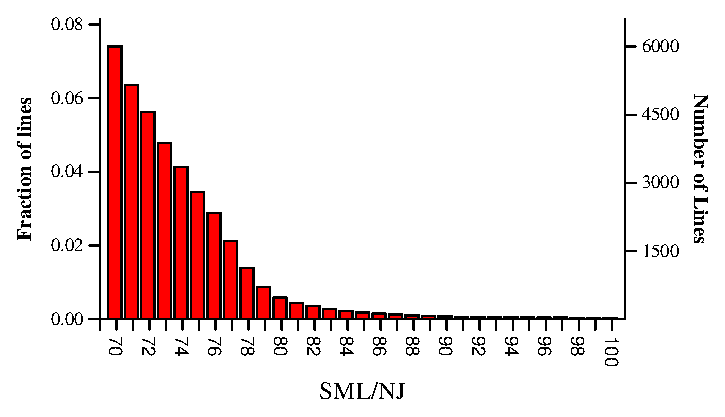
\includegraphics[scale=0.68]{smlnj.eps} & 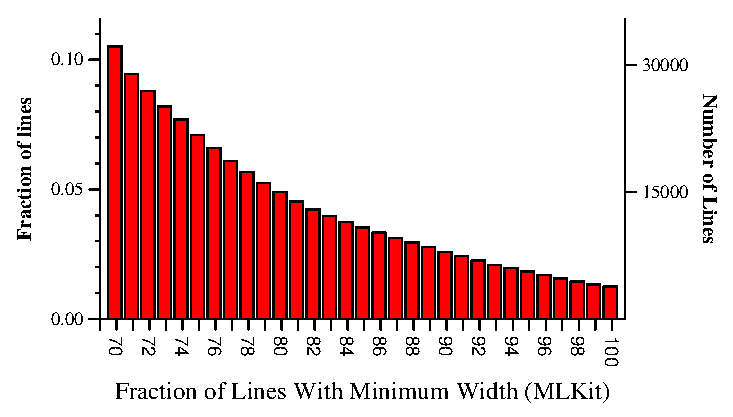
\includegraphics[scale=0.68]{mlkit.eps} \\
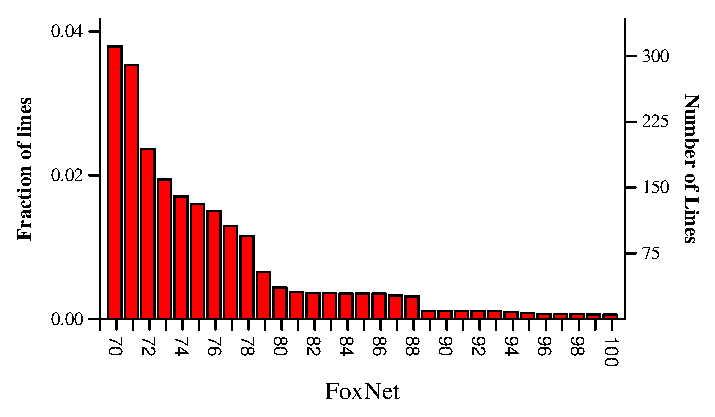
\includegraphics[scale=0.68]{foxnet.eps} & 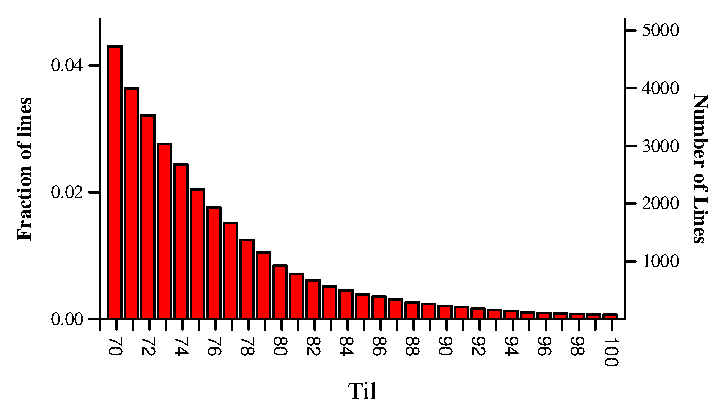
\includegraphics[scale=0.68]{til.eps} \\
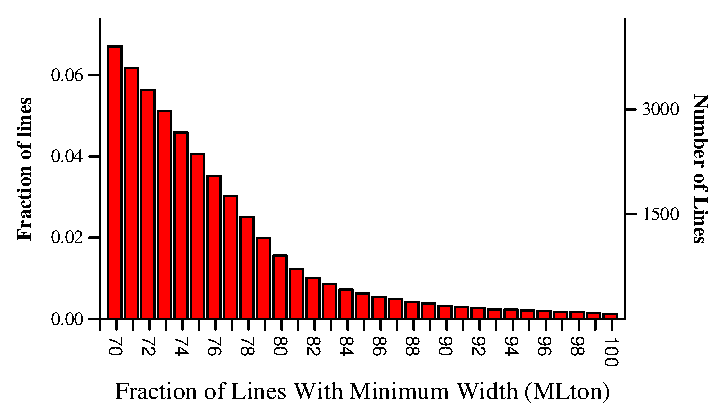
\includegraphics[scale=0.68]{mlton.eps} &
\end{tabular}
\caption{Fraction of lines and number of lines at least as wide as a given column limit}
\label{fig:width}
\end{figure}

Figure~\ref{fig:width} shows the results of our analysis
as an inverse cumulative histogram and an inverse cumulative density. In the SML/NJ project,
we notice an ``elbow'' in the plot around 80 columns. This inflection represents
an effort to limit the maximum width of lines. The tail of the inverse cumulative
histogram represents the failure to stay within the intended limit. We notice
also such as ``elbow'' in the MLton project, which we hypothesize
to mean that it also conforms generally to an 80-column limit.

FoxNet presents a more interesting profile in its inverse cumulative histogram. We see
two discontinuities: one at 80 columns and another at 88 columns, another popular width limit.
However, since there are so few lines in the FoxNet project, the data produced are
not as smooth as in other projects. We must therefore be careful not to attribute
artificial discontinuities caused by data discreteness to actual features. More
investigation on this required.

Finally, the MLKit project and Til project show no inflection in the
inverse cumulative histogram at all. This implies that the implementers of MLKit
and Til made little effort to limit line width at all!

Figure~\ref{fig:log-width} shows the same data plotted on a logarithmic scale.
We notice that the plots are quite linear ($R^{2} > 0.99$) for MLKit and Til.
This suggests an exponential decay in the number of violations as we increase the
threshold for violations. It certainly seems plausible that \emph{without} a
specified column limit, each increment in width limit results in a constant
fraction reduction in the number of violating lines.
Again, we have evidence that MLKit and Til do not employ column limits.
On the other hand, SML/NJ
and MLton exhibit a sigmoid when we look at their inverse cumulative histograms
on a logarithmic scale. The inflection at the center of the sigmoid corresponds to
the ``elbow'' mentioned before. We interpret this to mean that the coders are trying
to conform to some column limit since the fraction of lines falls more quickly near
the threshold than at smaller or larger limits. As before, it is difficult to
draw convincing conclusions from the FoxNet data because we are unsure
whether the features are real or simply an artifact of data discreteness.
\begin{figure}[h!]
\centering
\begin{tabular}{cc}
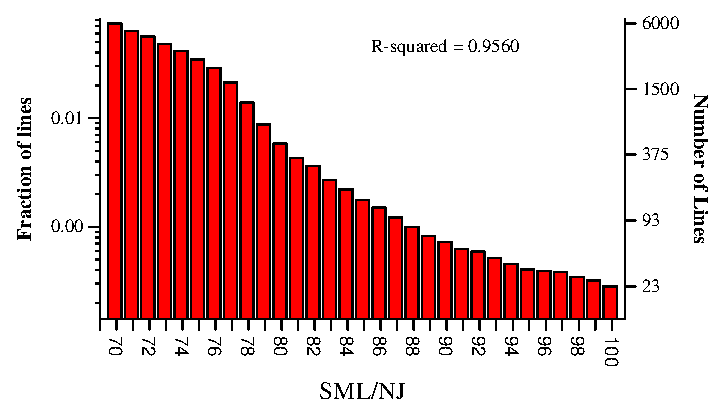
\includegraphics[scale=0.68]{log-smlnj.eps} & 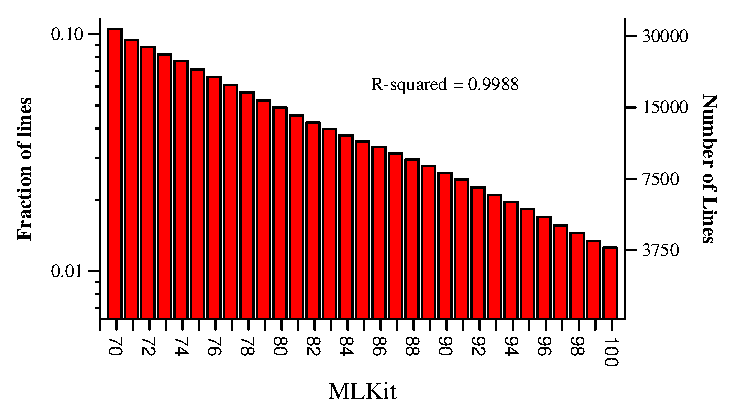
\includegraphics[scale=0.68]{log-mlkit.eps} \\
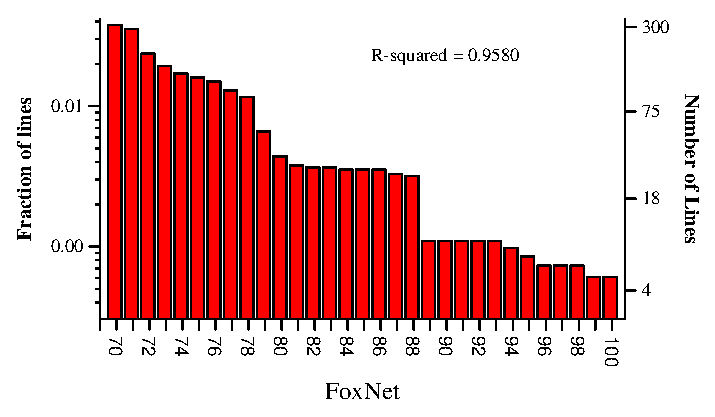
\includegraphics[scale=0.68]{log-foxnet.eps} & 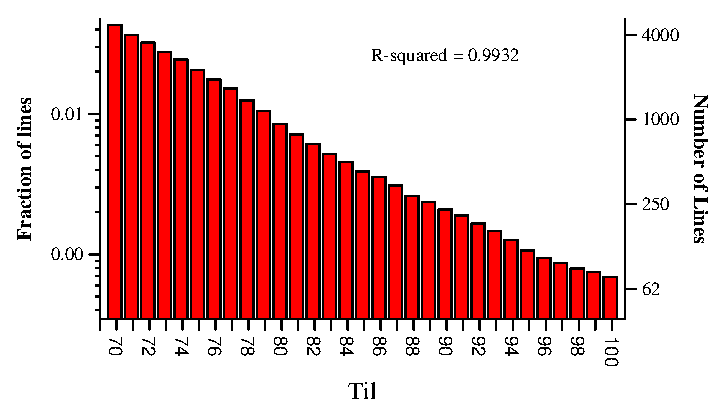
\includegraphics[scale=0.68]{log-til.eps} \\
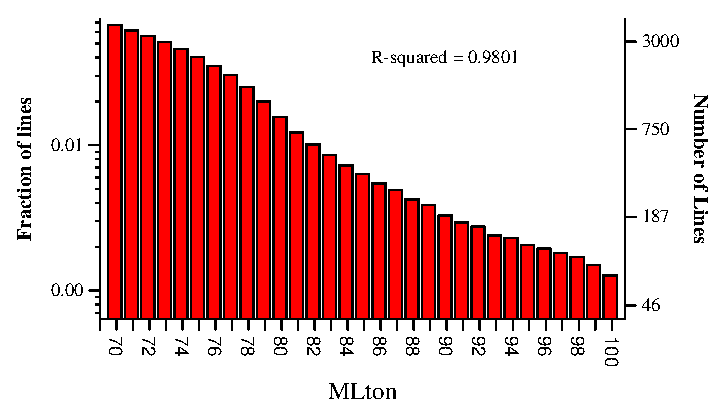
\includegraphics[scale=0.68]{log-mlton.eps} &
\end{tabular}
\caption{Log plot of fraction of lines and number of lines at least as wide as a given column limit. $R^{2}$ value shown for a least-squares linear fit of the logarithm.}
\label{fig:log-width}
\end{figure}

Clearly, not all experts conform to the 80-column rule.
Even those who appear to have an 80-column rule ignore it approximately 1\% of the time.
\subsection{Verbosity in \texttt{if} Expressions}
A convention cited in the Cornell style guide is that we should use \texttt{if}
expressions wisely. There are two specific uses of \texttt{if} that we
chose as violations.
\begin{enumerate}
\item Either one or both of the branches are boolean literals. We can rewrite the if expression with judicious use of \texttt{not}, \texttt{orelse}, and \texttt{andalso}
\item The test consists of \texttt{not} applied to another literal. We should just swap the two branches of the conditional.
\end{enumerate}
Rewriting these cases should help to improve readability and reduce verbosity in the code.

Table~\ref{table:style} shows the frequency of \texttt{if} violations in the five projects we selected.
There do not seem to be many violations -- on average approximately one every couple of thousand lines.
On inspection, the violations tend to fall into two groups: most are
missed opportunities to rewrite the \texttt{if} statement in potentially simpler way;
a few are made up of complicated \texttt{if} expressions where rewriting may not improve readability at all.
The first example below shows a \texttt{if} expression that could be rewritten as \texttt{e = t orelse f r}.
In the second case, the use of \texttt{orelse} does not significantly improve the readability or conciseness
of the expression. The problem is that the \texttt{if} expression has the same value as the test expression,
but if it evaluates to \texttt{false}, we also wish to evaluate some code for side effects.

\begin{figure}[h!]
\begin{enumerate}
\item \texttt{if e = t then true else f r}
\item \texttt{if ar1 = ar2 then true else (}$\langle$\emph{code with side effects}$\rangle$\texttt{; false)}
\end{enumerate}
\caption{Two \texttt{if} expressions from expert code where the \texttt{then} branch is the value \texttt{true}. In example 1, we could
rewrite in a more concise way by using \texttt{orelse}. In example 2, the use of \texttt{orelse} does not help much.}
\label{figure:ifthentrue}
\end{figure}

The expert code contains many uses of \texttt{orelse} and \texttt{andalso}, so we are forced to
conclude that the coders either missed an opportunity to use those syntactic constructs or chose
not to do so. Interestingly though, we do see \texttt{if} expressions of the following form:
\[\texttt{if }\langle expression\rangle\texttt{ then true else false}\]
There is one such example in the Til project, eight such examples in MLKit, and three instances
in SML/NJ. On inspection, there is no reason why each of these expressions could not be
rewritten by replacing the entire \texttt{if} expression with the test clause.
The test expressions are simple enough that it is unlikely that the authors
chose to use the \texttt{if} expression for reasons of increased legibility.
Instead, we suggest that the evidence points to omissions of carelessness.

\begin{table}[h!]
\centering
\begin{tabular}{|l||c|c|}\hline
Project & \texttt{if} violations & Lines per instance \\ \hline\hline
SML/NJ & 25 & 3244.1 \\
MLKit & 70 & 4373.6 \\
FoxNet & 0 & -- \\
Til & 23 & 4774.5 \\
MLton & 30 & 1940.9 \\ \hline
\end{tabular}
\caption{Instances of verbosity in \texttt{if} expressions (see text)}
\label{table:style}
\end{table}

\subsection{Fold}\label{subsec:fold}
The Cornell and CMU style guides both suggest making heaving use of library functions.
The author has noted, in discussions with the course staff for a programming languages course,
that beginners frequently overlook opportunities to
use library functions for lists. Since many of the basis functions
for lists, for example, \texttt{map}, \texttt{exists}, \texttt{all}, \texttt{filter},
and \texttt{rev}, can be written in terms of a fold over a list, we decided to look
for missed opportunities to apply a fold \cite{Jeu13}.
states that using higher order recursion schemes like a fold can allow a program
to benefit from shortcut fusion, and they
describe an algorithm for turning
explicitly recursive functions into folds.
We chose not to tackle the more challenging
problem of finding all fold opportunities or transforming them,
but instead chose to look for a specific
subset where folds might be applied.

Like \cite{Jeu13}, we are looking for cases of explicit recursion. Specifically, we try find
find instances of the following form:

\begin{figure}[!h]
\begin{center}
\texttt{fun f }\(e_{1}\ldots e_{i-1}\)\texttt{ (x::xs) }\(e_{i+1}\ldots e_{n}\)\texttt{=}\(e\)

where $e$ has the subexpression \texttt{f }\(v_{1}\ldots v_{i-1}\)\texttt{ xs }\(v_{i+1}\ldots v_{n}\)

And, either:

\texttt{fun f }\(e_{1}\ldots e_{i-1}\)\texttt{ [] }\(e_{i+1}\ldots e_{n}\) \texttt{= ...}

or

\texttt{fun f }\(e_{1}\ldots e_{i-1}\)\texttt{ \_ }\(e_{i+1}\ldots e_{n}\) \texttt{= ...}

\end{center}
\caption{A simplistic pattern for identifying explicit recursion that can be replaced with a fold}
\label{fig:folddef}
\end{figure}

That is, we're explicitly calling a recursive function on the tail of a input list.
The only other restriction is that the only list literal we allow in the same position
a declared pattern is the empty list literal (\texttt{[]}). This prevents idiosyncratic
behavior from being introduced into an otherwise sound definition by structural induction.
We won't concern ourselves with the order of the pattern match because either the patterns
are mutually exclusive (e.g., \texttt{[]} or a cons cell) or there is a redundant match
and the compiler will throw an error.
The motivation behind our definition is that a fold over a list in essence
a function that consumes a list. Explicit recursion defining this consumer must
consume a smaller list on each call, hence the requirement with a cons cell and a
call to the recursive function on the tail. In addition, we want our recursion to terminate
correctly, hence, the additional requirement that the function define a case that handles
the null list.
We, however, cannot claim to be able to identify all
fold opportunities correctly because of our inability to correctly parse infix expressions.

After performing an initial analysis, we looked at some
random samples of the violations we found.
Three are shown in Figure~\ref{fig:fold}.
A good number of these fold opportunities cannot actually
be written as fold because on encountering the null list, an error or
some other imperative code is executed. Example 1 falls under this category:
we see that the imperative function \texttt{bug} is executed
on a null list and potentially even as we are traversing the list.
Such a behavior cannot be captured by a fold because the value of a
fold on the null list defines the default accumulator and none
can be defined here.
That this example was found tells us that our search algorithm is unsound.

In example 2, we cannot use a fold because 
there is a recursive call on \texttt{xr'} instead of \texttt{xr},
which in essence, skips an element in the list traversal.
Fold, on the other hand, examines every element in the list.

Finally, in example 3, we see a example where we might consider
using the \texttt{exists} library function from the \texttt{List}
structure. While \texttt{exists} can be written as a fold,
it is inefficient to use a fold on a long list because
we cannot take advantage of the short-circuiting behavior
of the shown in this explicitly recursive function.

\begin{figure}
\begin{enumerate}
\item
\begin{verbatim}
fun try ((d as {name,rep,domain})::r) =
      (case rep of
         A.TAGGED i => if chk(gettag, i) then d else try r
       | A.CONSTANT i => if chk(Obj.toInt, i) then d else try r
       | A.TRANSPARENT => d
       | A.UNTAGGED => if Obj.boxed obj then d else try r
       | A.REF => d
       | A.LISTCONS => if (Obj.boxed obj) then d else try r
       | A.LISTNIL => if chk(Obj.toInt, 0) then d else try r
       | A.SUSP _ => d  (* LAZY *)
       | _ => bug "switch: funny datacon"
       (* end case *))
  | try [] = bug "switch: none of the datacons matched"
\end{verbatim}
\item
\begin{verbatim}
fun parseArgs [] acc = List.rev acc
  | parseArgs (x::xr) acc =
      if not (!state)
        then
          case keyword x
            of NONE => parseArgs xr acc
             | SOME Unknown => parseArgs xr (Data.Default x :: acc)
             | SOME (Eq a) => parseArgs xr (a::acc)
             | SOME f => case xr of
                           [] =>
                             raise
                               Data.BadArg (x ^ " takes one argument")
                         | (x'::xr') =>
                             parseArgs xr'
                               ((data x (toArgKind f) (next x x')) ::
                                   acc)
        else parseArgs xr (Data.Default x :: acc)
\end{verbatim}
\item
\begin{verbatim}
fun find (h :: t) = if h=index_n2 then true else find t
  | find nil =  false
\end{verbatim}
\end{enumerate}
\caption{Examples of ``missed fold opportunities''. Example 1 cannot be written as a fold
because there is not initial accumulator.
Example 2 can skip an element in the list
and is thus not condusive to translation into a fold. Example 3
can be written as a fold but would then not benefit from short-circuit testing.}
\label{fig:fold}
\end{figure}

We are forced to conclude that our simple framework for finding folds
is unfortunately unsound. The two primary reasons are that explicit recursion
can encode imperative behavior and provide behavior other than a simple
linear traversal of a list.
The problem with our simplistic pattern in Figure~\ref{fig:folddef}
is that we've failed capture the fact that a fold must have a well-defined
default accumulator and that it examines every element in a list.
So while it would be very helpful to identify places where we should
use a fold instead of explicit recursion, our approach does
not solve this problem.

We hoped to salvage something useful from this failed attempt.
Reviewers suggested that it is not always a good idea to transform
explicit recursion into a fold anyway, particularly if the accumulator becomes
too complex, but, they suggested, \texttt{map} and \texttt{filter}, which are
special cases of fold, are always preferable to explicit recursion.

We propose to identify opportunities for map and filter
in a similar fashion to how we identified opportunities for fold.
Here, in the recursive call, we look for the appearance of the cons operator (\texttt{::})
immediately before the function name. In addition, we desire for the
null list to appear as the right-hand side of one of the clauses.
Our analysis still lacks soundness since we are looking for
explicit recursion in the same manner. However, because we've stipulated
that the null list should occur on the right-hand side, we eliminate
the troublesome case where the starting value for the accumulator does not exist
(see example 1 in Figure~\ref{fig:fold}).

\begin{table}[h!]
\centering
\begin{tabular}{|l||c|c|}\hline
Project & \texttt{map}/\texttt{filter} violations & Lines per instance \\ \hline\hline
SML/NJ & 2 & 40551.0 \\
MLKit & 76 & 4028.34 \\
FoxNet & 2 & 4099.50 \\
Til & 4 & 27453.2 \\
MLton & 1 & 58226.0 \\ \hline
\end{tabular}
\caption{Missed opportunities to use map or filter}
\label{table:mapfilter}
\end{table}

Table~\ref{table:mapfilter} shows the results of the analysis.
Very few opportunities for using either map or filter exist.
Indeed, the experts are very keen on using these fold variants
instead explicit of explicit recursion.
This is particularly true with \texttt{map}, which we will show in section \ref{subsec:list}
is quite called quite frequently.
A random sampling of the violating declarations suggest that
these missed opportunities are generally truly missed opportunities.
Quite interestingly also, FoxNet seems to implement its own library
of utility functions, and our analysis found two of their
implementations of \texttt{filter} (\texttt{map} was not implemented).
While we cannot argue that our analysis is sound, we suggest it might
be a useful starting point for finding opportunities to apply
\texttt{map} and \texttt{filter}.
\subsection{Offside violations}\label{subsec:offside}
The \emph{offside rule} states that if a declaration or expression (or any language construct)
has to be split across multiple lines, later lines ought to be more indented relative to
the first line \cite{Lan66}.
The SML/NJ parser includes nodes with the name \texttt{MarkX} where \texttt{X} is
one of the syntactic categories (e.g., \texttt{MarkDec} for declaration, \texttt{MarkExp} for expression,
etc.). These are value constructors for the datatypes that represent the corresponding
syntactic category and their arguments indicate the character position for both the start and the
end of the enclosed syntactic structure. When we obtain a mapping from character position
to corresponding line and column within a source file (possible via the \texttt{SourceMap} structure),
we can attempt to examine the indentation of subexpressions or subdeclarations relative to
the indentations of their parents.

We ran into two complications with the analysis. The first is that when we have tabs present,
\texttt{SourceMap} treats the tab character has having a width of 1. Clearly,
this is not what we want. However, this problem is easily remedied 
by replacing tab characters with an equivalent number of spaces.
We can try to replace the tab with enough spaces such that
the last space ends on a column that is a multiple of 2, 4, or 8 (corresponding to those tab sizes)
and examine how the offside rule is followed in each set of replacements.

The more serious, and yet unsolved, complication is that if the first line of a construct
is indented, \texttt{SourceMap} returns the level of indentation
for the entire construct as the indentation for the first line.
Thus, if the first line of the construct is too far indented, all subsequent
lines get flagged for an offside violation, but the issue is most likely
with the incorrect indentation of the first line. We must address this
issue in future work before we can accurately report the number
of offside violations in the code.
\begin{figure}[bh!]
\centering
\begin{verbatim}
fun example x =
  let
      val _ = this line is indented too far to the right
    val _ = this line throws an offside violation
    val _ = so does this line
    ...
\end{verbatim}
\caption{Trouble detecting violations of the offside rule}
\label{fig:offside}
\end{figure}
\section{SYNTACTIC FORMS}\label{sec:syntax}
\subsection{Imperative Features}\label{subsec:imper}
One of the paradigms in writing functional programs is to avoid side effects.
Such a principled approach allows us to reason better about correctness and
removes the constraints imposed by having a fixed order of execution \cite{Hug90}. Therefore,
it behooves us to examine whether such imperative features are necessary or avoidable.

Any expression in ML can have a side effect. 
We are interested in expressions evaluated only for their side effects.
In Standard ML, there are two main constructs in terms of expressions that fit this mold:
(1)~the \texttt{while} expression and (2)~a list of expression separated by semicolons (similar to the \texttt{begin...end} syntax of Pascal) \cite{Ull98}.
The former has the form
\[\texttt{while <boolean-expression> do <expression>}\] and always returns a value of unit type.
The return value indicates that the \texttt{while} expression's purpose is to produce the side effects associated
with the expression in its body. The sequence of expressions evaluates only to the last in that sequence, indicating
in a similar fashion that all expressions in the list except for the last are evaluated only for side effects.

In addition, we can use the \texttt{val} declaration to assign the result
of an evaluation to unit or wildcard pattern. Again, the result of the evaluation
cannot be used, so the evaluation is performed only for side effects.
\begin{center}
\texttt{val () = ...}\\
\texttt{val \_ = ...}
\end{center}
\subsubsection{Expressions with \texttt{while}}
\begin{table}[h!]
\centering
\begin{tabular}{|l||c|c|}
\hline
Project & Instances of \texttt{while} & Lines per instance \\ \hline\hline
SML/NJ & 0 & --\\
MLKit & 0 & --\\
FoxNet & 0 & -- \\
Til & 2 & 54906.5 \\
MLton & 0 & --\\ \hline
\end{tabular}
\caption{Occurrences of \texttt{while} expressions}
\label{table:while}
\end{table}
As we can see from Table~\ref{table:while}, only the Til
project uses \texttt{while} loops.
In the two instances found in the Til project, the body of the \texttt{while}
loop includes modifying a mutable reference, which justifies the use of
an imperative feature. Getting rid of the while loops requires a design of how the code works so
that we no longer need to keep track of mutable state and thus, is not very straightforward.

Overall, we can observe that there are very few usages of \texttt{while} expressions
in expert projects.
From the analysis, expert ML programmers seemed quite principled in avoiding imperative
elements of ML. This is perhaps not surprising since they could have chosen
to implement in any language but selected a functional language in the end.
\subsubsection{Expression Lists}
\begin{table}[h!]
\centering
\begin{tabular}{|l||c|c|}
\hline
Project & Instances of expression lists & Lines per instance \\ \hline\hline
SML/NJ & 1,970 & 41.17 \\
MLKit & 3,869 & 79.13 \\
FoxNet & 68 & 120.6 \\
Til & 1,928 & 59.96 \\
MLton & 641 & 90.84 \\ \hline
\end{tabular}
\caption{Occurrences of expressions lists}
\label{table:explist}
\end{table}
Table~\ref{table:explist} shows how often expression lists are used in our
examples of expert ML code. We find that the number of uses is significantly
greater than that of the \texttt{while} expression. The greatest number
of occurrences, normalized by the number of lines, appears to be in the SML/NJ
compiler where we find an expression list on average once every with every
40 or so lines of code.

The expression lists are likely used for the side effects of the non-terminal
expression in the list. Sadly, the expressions are quite complex and difficult
to aggregate into meaningful groupings programmatically. Nevertheless,
looking at the examples of expression lists in the expert code, we find that
the expression lists frequently occur in the following contexts:
\begin{itemize}
\item[$\bullet$] pretty printing
\item[$\bullet$] outputting error messages
\item[$\bullet$] other types of I/O
\item[$\bullet$] assignment of reference variables (with \texttt{:=})
\item[$\bullet$] arrays
\item[$\bullet$] with the keyword \texttt{use} or the compilation manager to bring in other modules
\end{itemize}

Haskell has the IO monad to allow users to perform I/O in a purely functional way \cite{Jon93}.
Standard ML does not, so users are left to perform their
I/O in imperative fashion.

Arrays and references are two examples that \cite{Ull98} cites as way to ``violate the functional,
side-effect-free style,'' but also noting that ``there are situations where programs cannot
be made adequately efficient unless we are allowed to change some value bindings.''
\subsubsection{Unit \texttt{val} and wildcard \texttt{val}}
\begin{table}[h!]
\centering
\begin{tabular}{|l||c|c|}
\hline
Project & Instances of imperative \texttt{val} & Lines per instance \\ \hline\hline
SML/NJ & 296 & 273.99 \\
MLKit & 532 & 575.48 \\
FoxNet & 70 & 117.13 \\
Til & 427 & 257.17 \\
MLton & 731 & 79.653 \\ \hline
\end{tabular}
\caption{Occurrences of imperative \texttt{val} bindings}
\label{table:val}
\end{table}

Table~\ref{table:val} shows that imperative \texttt{val} bindings
occur with frequency comparable to that of expression lists.
Indeed, most of these occurrences are also for the purpose of I/O.
Therefore, we conclude that experts use imperative \texttt{val} bindings
to achieve execute one-time imperative code.
\subsubsection{Final thoughts on imperative features}
Imperative features are clearly unavoidable as evidenced in expert ML code. The experts do
limit their uses of expression lists to a few general cases, mostly dominated by I/O.
We conclude that the ML experts believe in the ``functional, side-effect-free'' style
and conform to it as much as possible. Beginners in ML are encouraged for follow their example.
\subsection{List Library Functions}\label{subsec:list}
We wanted to see if there was any discernable pattern in how expert programmers
used library functions, but not all projects require the same library.
It is difficult to imagine writing a substantial amount of code in ML without
relying heavily on lists, so we decided to examine how much expert programmers relied upon the functions
in the \texttt{List} structure from the standard basis.

\begin{table}[h!]
\centering
\begin{tabular}{|l||c|c|c|c|c||c|}
\hline
Function & SML/NJ & MLKit & FoxNet & Til & MLton & Mean fraction of calls \\ \hline\hline
\texttt{::} & \textbf{882} & \textbf{6,350} & \textbf{97} & \textbf{801} & \textbf{372} & 0.3743 \\
\texttt{map} & \textbf{701} & \textbf{1,724} & \textbf{60} & \textbf{1,029} & \textbf{108} & 0.2150 \\
\texttt{@} & \textbf{205} & \textbf{602} & \textbf{18} & \textbf{248} & \textbf{69} & 0.0688 \\
folds & \textbf{237} & \textbf{920} & \textbf{15} & \textbf{171} & \textbf{57} & 0.0664 \\
\hspace{0.2in}\texttt{foldl} & 89 & 522 & 7 & 59 & 30 & 0.0304 \\
\hspace{0.2in}\texttt{foldr} & \textbf{148} & 398 & 8 & 112 & 27 & 0.0360 \\
\texttt{app} & \textbf{331} & \textbf{728} & 3 & \textbf{340} & \textbf{45} & 0.0664 \\
\texttt{rev} & 137 & 472 & \textbf{13} & \textbf{178} & \textbf{120} & 0.0627 \\
\texttt{length} & \textbf{163} & 578 & 3 & 119 & \textbf{87} & 0.0471 \\
\texttt{tl} & 54 & 114 & 0 & \textbf{171} & 26 & 0.0207 \\
\texttt{hd} & 42 & 44 & 0 & 133 & 16 & 0.0146 \\
\texttt{all} & 13 & 76 & 0 & 53 & 35 & 0.0119 \\
\texttt{find} & 48 & 130 & 0 & 48 & 13 & 0.0107 \\
\texttt{exists} & 24 & 96 & 0 & 25 & 28 & 0.0100 \\
\texttt{filter} & 17 & 138 & 3 & 4 & 8 & 0.0080 \\
\texttt{last} & 8 & 78 & 0 & 2 & 22 & 0.0061 \\
\texttt{null} & 8 & 50 & 0 & 1  & 20 & 0.0052 \\
\texttt{tabulate} & 1 & 18 & 0 & 0  & 13 & 0.0028 \\
\texttt{nth} & 5 & 4 & 0 & 6 & 8 & 0.0023 \\
\texttt{partition} & 14  & 14 & 0 & 3 & 2 & 0.0018 \\
\texttt{mapPartial} & 7 & 26 & 0 & 0 & 3 & 0.0015 \\
\texttt{take} & 6 & 10 & 0 & 10 & 1 & 0.0014 \\
\texttt{drop} & 0 & 28 & 0 & 7 & 2 & 0.0013 \\
\texttt{getItem} & 0 & 20 & 0 & 0 & 2 & 0.0007 \\
\texttt{revAppend} & 1 & 0 & 0 & 0 & 1 & 0.0003 \\
\hline\hline
Total & 2,904 & 12,220 & 212 & 3,349 & 1,058 & \\
Lines per call & 27.928 & 25.054 & 38.674 & 32.790 & 55.034 & \\\hline
\end{tabular}
\caption{Calls to functions from the \texttt{List} structure (\texttt{concat} omitted) ordered by the average
fraction of calls that each function contributes in the five projects.
Bolded entries each account for more than 5\% of the total number of occurrences in a project.}
\label{table:list}
\end{table}

Since the easiest way to create lists of arbitrary size is to the use the cons operator (\texttt{::}),
this operator naturally occurs the most, accounting for, in some cases, half
the occurrences of function calls. But we don't gain much insight from looking at this operator
because it is so common and critical to working with lists. It should also be noted
that we are excluding any occurrences of the cons operator used in pattern matching.
Additionally, we had trouble distinguishing uses of \texttt{concat} from the \texttt{List} structure
as opposed to the \texttt{String} structure. As a result, the occurrences of \texttt{concat} have been omitted.
Our results are tabulated in Table~\ref{table:list}.

It is amazing that list functions are used with almost the same frequency (normalized
by the number of lines) in every expert project. The normalized frequency
basically stay constant, relative to each other, even when we exclude the occurrences of the cons operator.

The values in bold indicate that a function accounts for more than 5\% of all function calls to the \texttt{List} structure.
We see that folds (both left and right), list concatenation (\texttt{@}), and \texttt{map} break the threshold in all 5 projects. Between them,
\texttt{map} is more common, with a frequency matching the cons operator in some cases.
This suggests possibly that expert coders in ML are transforming data in bulk within a list container.
Indeed, outside of the cons operator, \texttt{map} seems to be by far the most common function called
from the \texttt{List} structure.

The pair of fold functions, taken together, break the threshold on all five projects.
This is perhaps not surprising since a fold is an excellent way to aggregate data in a list
into another value, possibly even another list. Indeed, many of the functions on lists
including \texttt{map} could be rewritten using a fold.

Another function of note is \texttt{app}, which each accounts for more than 5\% of
occurrences in four of five projects. The \texttt{app} is particularly interesting because it can be
considered an imperative version of \texttt{map}, which we have observed is called quite often. We hypothesize
that not only do expert programmers transform data in bulk as a list with \texttt{map}, the execute side effects
in bulk in a list with \texttt{app}.

Finally, we point out that \texttt{hd} and \texttt{tl} account for, on average, only about 2\% of all
function calls. Only in Til does \texttt{tl} exceed our 5\% threshold (and just barely at 5.1\%).
The \texttt{hd} and \texttt{tl} functions respectively return the first element and all but the first element in a list.
That they are used relatively infrequently is interesting because from
the author's experience, extracting the head and tail of a list is unavoidable in practice.
It is likely that expert coders prefer pattern matching on a cons cell (e.g., \texttt{x ::\ xs})
instead of explicitly calling either \texttt{hd} or \texttt{tl}.
\subsection{Program Hierarchy and Layout}\label{subsec:struct}
\subsubsection{Modularity and Abstraction}\label{subsubsec:modularity}
Program modularity eases the burden of maintenance and refactoring.
Abstraction provides a uniform interface, hides distracting implementation details,
and conceals sensitive information. With ML's module system, we can achieve
abstraction and modularity by using structures, signatures, and functors.

\begin{table}[h!]
\centering
\begin{tabular}{|l||>{\centering\arraybackslash}p{1.5in}|c||>{\centering\arraybackslash}p{1.5in}|c|}
\hline
Project & Files with module declarations & Fraction & Files with only module declarations & Fraction \\ \hline\hline
SML/NJ & 297 & 0.99 & 297 & 0.99 \\
MLKit & 1,308 & 0.99 & 1,270 & 0.96 \\
FoxNet & 30 & 0.42 & 29 & 0.40 \\
Til & 445 & 0.97 & 443 & 0.96 \\
MLton & 397 & 0.94 & 386 & 0.91 \\ \hline
\end{tabular}
\caption{Proportion of files that, at top level, contain module declarations or only contain module declarations.}
\label{table:module}
\end{table}

Table~\ref{table:module} shows what fraction of files define a structure, signature, or functor at top level
and what fraction of files define only a structure, signature, or functor at top level.
We find that in larger projects, almost every single file contains a functor, signature, or structure
definitions at top level. Nearly as many have at least one such declaration in a file.
The smaller FoxNet project stands out as having a smaller fraction in both cases.

We believe that these data reflect that as projects get large, expert ML coders
make very heavy use of the ML module system to help manage the complexity.
Due to the experts' heavy reliance on the ML module system,
we suggest to beginners to also make good use of the ML module system
to impart modularity and some level of abstraction to their work, particularly
when the projects they are working on grow in size.
\subsubsection{Helper Functions in \texttt{let} Expressions and \texttt{local} Declarations}\label{subsubsec:let}
Helper functions allow programmers to refer to recurring code by name.
They can also help make the code more readable by giving complicated
lambda expressions a helpful name. We might consider looking at
how frequently our expert examples employ helper functions. Sadly,
we cannot infer from the name of a function or its body whether or not
a function is a helper function. But if a function appears inside
the list of declarations in a \texttt{let} expression or a \texttt{local}
declaration, one might hypothesize that it is likely a helper function
of some sort, since its scope is limited to the body of the \texttt{let}
or \texttt{local} construction.

\begin{table}[h!]
\centering
\begin{tabular}{|l||>{\centering\arraybackslash}p{1.2in}|>{\centering\arraybackslash}p{1.2in}|c||>{\centering\arraybackslash}p{1.2in}|c|}
\hline
Project & Function declarations in \texttt{let} & Function declarations in \texttt{local} & Sum & Total Function Declarations & Fraction \\ \hline\hline
SML/NJ & 2,652 & 192 & 2,844 & 4,866 & 0.58 \\
MLKit & 6,130 & 2,682 & 8,812 & 24,841 & 0.35 \\
FoxNet & 103 & 19 & 122 & 530 & 0.23 \\
Til & 1,856 & 500 & 2,356 & 5,627 & 0.42 \\
MLton & 1,004 & 252 & 1,256 & 3,533 & 0.36 \\\hline
\end{tabular}
\caption{Functions declared inside of \texttt{let} expressions}
\label{table:funlet}
\end{table}

Table~\ref{table:funlet} shows how functions are declared inside of \texttt{let} or \texttt{local}
constructs, and what fraction that represents out of all function declarations in the
entire project.
In the larger four projects, at least one-third of all function declarations occur
inside of a local or a let binding. As argued above, these are likely to be helper functions.
The experts are quite fond of helper functions if one out of every three functions
are helper functions. Beginners are encouraged for follow their example.
\section{MAKING SENSE OF RECOMMENDATIONS}\label{sec:rec}
Instead of having a veritable witch's brew of recommendations for beginners,
we thought it might be useful to group them into categories both to
organize the concepts and because research has shown that grouping items into
``chunks'' helps memory and learning \cite{Gob01}.

In retrospect, we see that all of our recommendations touch on the structure of
an ML program in some way, and we can classify the recommendations as dealing
with (1)~typographic structure, (2)~syntactic structure, or (3)~organizational structure.
\subsection{Typographic Structure}
By typographic structure, we mean how the code physically looks and the mechanisms
used to enhance or emphasize visualization. The typographic structure rules are:
\begin{enumerate}
\item There is no general consensus on tabs vs.\ spaces. Pick one and be consistent.
\item Try to keep under 80 columns of text, but it's OK go over occasionally.
\end{enumerate}
Typographic structure is important because it makes code easier to read and therefore
easier to understand.
\subsection{Syntactic Structure}
Syntactic structure covers when and what syntactic elements and features of ML to use
in a source file. These rules are derived from expert choices in the same
situations and are likely motivated by reasons of code legibility and efficiency:
\begin{enumerate}
\item Rewrite if expressions if one of the branches is a boolean literal or if the test is \texttt{not} applied a boolean expression
\item Folds are nice if appropriate, but experts almost always use \texttt{map} and \texttt{filter} when given the option.
\item Avoid \texttt{while} loops.
\item Expression lists are OK for I/O.
\item Imperative \texttt{val} bindings are OK for I/O.
\item Use list library functions when possible, especially \texttt{map} and folds.
\item Pattern match on lists instead of using \texttt{hd} or \texttt{tl}
\end{enumerate}
\subsection{Organizational Structure}
Organizational structure is intended to mean how code is organized at high levels.
Thus, the use of helper functions and the module system fall under this category.
Expert projects can be daunting both in terms of size and complexity, so good
organization is key. These rules are derived from observing how experts organize their code:
\begin{enumerate}
\item Modularize your code with structures, signatures, and functors.
\item Use helper functions.
\end{enumerate}
\section{CONCLUSIONS AND CONTRIBUTIONS}\label{sec:future}
The key contributions of this project are three-fold. First, we
identified some features of ML expertise. These features are
selected not based on what experts recommend but rather on how they
write their own code. This is also the key area for future work
because there are certainly many more features that could be examined.

Second, we've distilled some useful rules for novices based
on our discoveries and organized them into categories
to better aid understanding and application of these rules.

Finally, we've created a set of tools that programmers of all levels
can use to evaluate how well they are performing on the above
eight points. The primary audience is intended to be novices,
who can receive feedback on how well certain features
of their code mirror those of experts. As more features are examined
in future work, the tools will certainly be expanded to cover those
features.
\section*{SOURCE CODE}
The source code is available on GitHub via \url{http://www.github.com/zhelu/smlproject}.
\begin{thebibliography}{99}
\bibitem[Ayerbe and Vazquez 1998]{Aye98} Ayerbe, A., Vazquez, I. (1998) Software Products Quality Improvement with a Programming Style Guide and a Measurement Process. In \emph{Proceedings 22nd Annual International Computer Software and Applications Conference (COMPSAC'98)}. 172--178.
\bibitem[Binkley 2007]{Bin07} Binkley, D., 2007. Source Code Analysis: A Road Map. In \emph{Workshop on the Future of Software Engineering (FOSE'07)}. Minneapolis, MN. 104--119. Washington, D.C.: IEEE Computer Society.
\bibitem[Bouwers et al. 2012]{Bou12} Bouwers, E., Visser, J., van Deursen, A. (2012) Getting what you measure. \emph{Commun. ACM}, \textbf{55}, 54--59.
\bibitem[CMU 2012]{Cmu12} CMU Computer Science Department. (2012) SML Style Guide. Accessed on 14 Nov 2013 from \url{http://www.cs.cmu.edu/~15150/resources/style.pdf}
\bibitem[Ericsson et al. 1993]{Eri93} Ericsson, K.\,A., Krampe, R.\,T., Tesch-R\"{o}mer, C. (1993) The Role of Deliberate Practice in the Acquisition of Expert Performance. \emph{Psychological Rev.} \textbf{100}, 363--406.
\bibitem[Gladwell 2008]{Gla08} Gladwell, M. (2008) \emph{Outliers}. Little, Brown and Co., New York, NY.
\bibitem[Gobet et al. 2001]{Gob01} Gobet, F., Lane, P.\,C.\,R., Croker, S., Cheng, P.\,C-H., Jones, G., Oliver, I., Pine, J.\,M. (2001) Chunking mechanism in human learning. \emph{Trends in Cognitive Sci.} \textbf{5}, 236--243.
\bibitem[Hughes 1990]{Hug90} Hughes, J. (1990) Why Functional Programming Matters. In D.\,A.\,Turner, ed, \emph{Research Topics in Functional Programming}. Boston, MA: Addison-Wesley.
\bibitem[Jones 1994]{Jon94} Jones, C. (1994) Software metrics: good, bad and missing. \emph{Computers}, \textbf{27}, 98--100.
\bibitem[Kernighan and Plauger]{Ker78} Kernighan, B.\,W., Plauger, P.\,J. (1978) \emph{The Elements of Programming Style}. New York, NY: Yourdon.
\bibitem[Landin 1966]{Lan66} Landin, P. (1966) The Next 700 Programming Languages. \emph{Comm. ACM}, \textbf{9}, 157--166.
\bibitem[Ordonez and Hadda 2008]{Ord08} Ordonez, M.\,J. Hadda, H.\,M. (2008) The State of Metrics in Software Industry. In \emph{5th International Conference Information Technology: New Generations (ITNG'08)} Las Vegas, NV. 453--458. Washington, D.C.: IEEE Computer Society.
\bibitem[Peyton Jones, Wadler 1993]{Jon93} Peyton Jones, S.\,L., Wadler, P. (1993) Imperative Functional Programming. In \emph{ACM Symposium on Principles of Programming Languages (POPL'93)}. Charleston, SC. 71--84. New York, NY: ACM.
\bibitem[Takai et al. 2011]{Tak11} Takai, Y., Kobayashi, T., Agusa, K. (2011) Software Metrics Based on Coding Standards Violations. In \emph{2011 Joint Conference of the 21st Int'l Workshop on Software Measurement and 6th Int'l Conference on Software Process and Product Measurement (IWSM-MENSURA)} Nara, Japan. 273--278. Washington, D.C.: IEEE Computer Society.
\bibitem[Ullman 1998]{Ull98} Ullman, J.\,D. (1998) \emph{Elements of ML Programming} (ML97 Ed). Prentice Hall, Upper Saddle River, NJ.
\bibitem[Van der Jeugt et al. 2013]{Jeu13} Van der Jeugt, J., Keuchel, S., Schrijvers, T. (2013) Bringing Functions into the Fold. Unpublished manuscript.
\bibitem[Vogelsang et al. 2010]{Vog10} Vogelsang, S., Fehnker, A., Huuck, R., Reif, W. (2010) Software Metrics in Static Program Analysis. In \emph{Formal Methods and Software Engineering. Proceedings 12th International Conference on Formal Engineering Methods (ICFEM'10)}. Shanghai, China. 485--500. Heidelberg, Germany: Springer.
\end{thebibliography}
\end{document}
